\chapter{Stand van zaken}
\label{ch:stand-van-zaken}

% Tip: Begin elk hoofdstuk met een paragraaf inleiding die beschrijft hoe
% dit hoofdstuk past binnen het geheel van de bachelorproef. Geef in het
% bijzonder aan wat de link is met het vorige en volgende hoofdstuk.

% Pas na deze inleidende paragraaf komt de eerste sectiehoofding.

\section{Machine Learning}
\label{sec:Machine Learning}
Machine learning is een vakgebied binnen artificiële intelligentie dat het mogelijk maakt om presentaties van een systeem te verbeteren op basis van voorbeeldgegevens of ervaringen uit het verleden. Het biedt computers de mogelijkheid om te leren zonder expliciet geprogrammeerd te zijn \autocite{Spark}.
Sommige taken of problemen kunnen niet voorafgaand geprogrammeerd worden. Vaak zijn ze te complex en onpraktisch om rechtstreeks door mensen gecodeerd te worden. Evenwel wordt het moeilijk om in een veranderende omgeving een programma te ontwikkelen die optimaal werkt omdat bepaalde kenmerken van de omgeving niet bekend zijn tijdens het ontwerp \autocite{Stanford}.

Gebrek aan kennis wordt bij machine learning goedgemaakt door data. Op basis van een groot aantal voorbeelden kan een model gedefinieerd worden om voorspellingen te doen of om kennis te verzamelen.  Een voorbeeldtoepassing hiervan is een spamfilter. Om reden dat spam veranderd met de tijd en verschilt van persoon tot persoon is het ingewikkeld om een specifiek algoritme te ontwikkelen die spam e-mails onderscheidt van geldige e-mails. De bedoeling is dat een computer automatisch een algoritme uitwerkt om spam te herkennen op basis van duizenden gekende spam e-mails en geldige e-mails \autocite{Alpaydin}.
Verder wordt machine learning gebruikt in allerhande toepassingen in verschillende sectoren. Zo gebruikt Netflix en Spotify een aanbevelingsalgoritme om hun klanten te voorzien van films respectievelijk muziek die ze waarschijnlijk leuk vinden. Daarnaast gebruikt Paypal dergelijke algoritmes om fraude te detecteren \autocite{Redpixie}.

Door het veelzijdig gebruik van machine learning algoritmes met verschillende doelstellingen kan het onderverdeeld worden in drie hoofdcategorieën: Supervised learning, Unsupervised learning, Reinforcement learning.


\subsection{Supervised Learning}
\label{ssec:Supervised Learning}
Supervised machine learning bouwt een model steunend op een reeks invoergegevens waarvan de uitvoer gekend is. Bij de uitvoer wordt er onderscheidt gemaakt tussen regressie, waar het resultaat een numerieke waarde is en classificatie waar kwalitatieve waarde is zoals een klasse of een label. Een regressietaak is bijvoorbeeld het voorspellen van de wisselkoers. Een classificatie opdracht moet dan weer onderscheidt maken tussen bier en wijn op basis van het kleur en alcoholgehalte. Het supervised algoritme gebruikt de bekende invoergegevens om voorspellingen te genereren voor de uitvoer van nieuwe gegevens. Het algoritme kan steeds verder getraind worden door het toevoegen van voorbeeldgegevens tot het een acceptabel nauwkeurigheidsniveau heeft bereikt \autocite{Dummies}.

\subsection{Unsupervised Learning}
\label{ssec:Unsupervised Learning}
Wanneer er enkel invoerdata beschikbaar is, is er sprake van unsupervised learning. Het algoritme gaat opzoek naar verborgen patronen of onbekende structuren in de gegevens. Het heeft als doel om bruikbare informatie uit een set van invoergegevens te halen. Voor mensen is dit type alogritme nuttig om inzicht te krijgen in een groep verzamelde gegevens. De meest voorkomende techniek is clustering, het verdeeld de gegeven data in gelijkaardige groepen. Het groeperen van klanten op basis van het koopgedrag is een veelgebruikt voorbeeld van clustering \autocite{Mathworks}.

\subsection{Reinforcement Learning}
\label{ssec:Reinforcement Learning}
Wanneer reinforcement learning van toepassing is, dan leert een machine uit zijn voorheen genomen acties. Elke actie is verbonden met een resultaat dat positief of negatief kan zijn. Neemt een machine een verkeerde actie, dan levert dit een kost op. Een goede actie levert een beloning op. Het algoritme leert continu op een iteratieve manier van de omgeving en zijn ondernomen beslissingen met als doel het maximaliseren van de beloning op lange termijn. Reinforcement learning wordt gebruikt om computers zelf aan te leren om videogames te spelen \autocite{incompleteideas}.

\section{Deep Learning}
\label{sec:Deep Learning}
Deep learning is een onderdeel van machine learning die gebruikt maakt van algoritmes die gebaseerd zijn op de structuur van het menselijk brein. Klassieke machine learning technieken zijn beperkt in hun capaciteit om gegevens te verwerken. Tussen de invoer en het resultaat zit doorgaands een enkele verwerkingslaag die gebruikt worden voor voorspellingen of classificatie.  Diep learning verwerkt de invoer op meerdere niveaus met toenemende complexiteit en abstractie. Elke verborgen laag in de hiërarchie past een transformatie toe op de uitvoer van de voorgaande laag tot het een aanvaardbaar maat van nauwkeurigheid heeft bereikt. Bij elke iteratie wordt het model dat de computer ontwikkeld dus complexer maar ook nauwkeuriger. Het grote voordeel hierbij is dat het algoritme zichzelf aanleert om laag per laag aspecten van de input te herkennen \autocite{toronto}.

Als voorbeeld wordt een analogie uit het dagelijkse leven aangehaald. Een peuter leert wat een kat is door naar dieren te wijzen en het woord kat uit te spreken. De ouder corrigeert de peuter wanneer hij naar een foutief dier wijst. Na verloop van tijd wordt de peuter zich meer en meer bewust van de kenmerken die een kat heeft. Hij bouwt een hiërarchie op van verschillende lagen waarin elk niveau van abstractie gecreeërd wordt met de kennis die  opgenomen is uit de voorgaande laag. Deep learning algoritmes doorgaan hetzelfde proces. Het ontvangt een gegevensset waarvan geweten is of het al dan niet een kat is. Daarna wordt de elke input getransformeerd naar een volgend niveau om zo patronen te herkennen.  In de eerste laag wordt bijvoorbeeld gezocht naar de aan- of afwezigheid van randen op bepaalde locaties in het beeld. In de tweede laag kunnen als voorbeeld vormen gedetecteerd worden zoals oren en poten. Zo wordt de input zodanig getransformeerd totdat het model nauwkeurigheid genoeg is om voorspellingen te doen \autocite{techtarget}.

Het doel van deep learning is de werking van het menselijk brein zo goed mogelijk te reproduceren. Er zijn al heel wat applicaties die gebruikmaken van deep learning algoritmen. Afbeelding- en spraakherkenning zijn de meest voorkomende toepassingen. Maar ook het automatisch inkleuren van zwartwit foto’s en zelfrijdende auto’s maken gebruik van d

\section{Convolutional Neural Network}
\label{sec:Convolutional Neural Network}

Een convolutional neural network, afgekort CNN is een supervised deap learning algoritme dat vooral gebruikt wordt voor beeld- en videoherkenning. Ook voor het classificeren van afbeeldingen wordt een CNN gebruikt. Het netwerk krijgt hierbij een afbeelding als input en geeft de waarschijnlijkheid dat de afbeelding tot een klasse behoort terug als resultaat. De input kan hierbij aanzien worden als een drie dimensionale array van pixels. Een afbeelding met een grootte van 20 bij 20 pixels heeft een array van 20 x 20 x 3 pixels. De diepte 3 is omwille van de drie kleurkanalen rood, groen en blauw. Voor elk kanaal is er een twee dimensionale array waarbij elke pixel een waard heeft tussen 0 en 255. Bij een zwart-wit beeld is de diepte vanzelfsprekend gelijk aan 1. In dit netwerk bestaan de verborgen lagen uit een aantal convolutional, nonlinair, pooling en fully connected layers \autocite{brohrer}. Figuur \ref{fig:structuur} geeft de grafische voorstelling hoe een CNN is opgebouwd weer.  
\begin{figure}
    \centering
        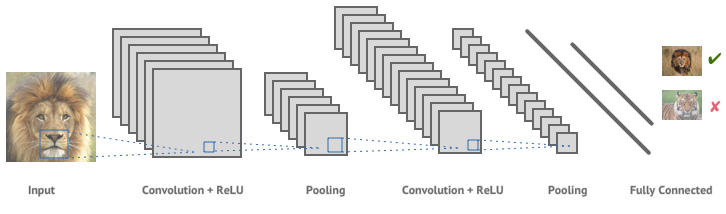
\includegraphics[width=1\textwidth]{img/convolutional_neural_network.png}
    \caption{Typische structuur van een Convolutional Neural Network \autocite{tejani}}
    \label{fig:structuur}
  \end{figure}

\subsection{Convolutional Layer}
\label{ssec:Convolutional Layer}
De eerst verborgen laag in een CNN is een convolutional layer. In deze laag wordt elk deel van de afbeelding vermenigvuldigd door bepaalde filters, een filter schuift of convoleert als het ware over de afbeelding. De bedoeling van een filter is om een feature of kenmerk te detecteren in een afbeelding. Dit kan gaan van eenvoudige herkenbare vormen zoals randen en bepaalde curves tot complexere structuren zoals ogen en oren. Het resultaat van de vermenigvuldiging geeft een quotering in hoeverre de feature aanwezig is. Nadat de filter over alle locaties van de invoer heeft geschoven vormen alle resultaten één nieuwe matrix. In de convulotional layer wordt één afbeelding omgezet naar een groep gefilterde afbeeldingen, afhankelijk van het aantal filters. Deze output wordt de input voor de volgende verborgen laag \autocite{becominghuman}.
Figuur \ref{fig:featuremap} toont een mooi voorbeeld van een feature map waarbij de filter randen detecteerde op een afbeelding van een tijger.
\begin{figure}[h!]
    \centering
        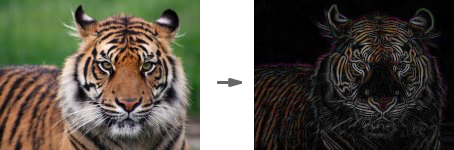
\includegraphics[width=0.5\textwidth]{img/tiger_edge_detection.png}
    \caption{Originele afbeelding gefilterd naar een feature map \autocite{tejani}}
    \label{fig:featuremap}
  \end{figure}

\subsection{Nonlinair Layer}
\label{ssec:Nonlinair Layer}
Deze laag ontvangt als input een verzameling van gefilterde afbeeldingen of ‘feature maps’. Aangezien de filter of functie uit de vorige laag linair is, kan het resultaat op een deel van de afbeelding ook negatief zijn. De nonlinair layer zet de linaire convolutielaag om naar een niet-linaire laag door een gelijkrichterfunctie, ReLu (Rectified Linear Unit) toe te passen. Deze functie zet alle negatieve waarden om naar de nulwaarde \autocite{cadence}.

\subsection{Pooling Layer}
\label{ssec:Pooling layer}
Pooling, of ook wel subsampling genoemd wordt gebruikt om de dimensie of grootte van de feature maps te verkleinen. In deze laag wordt het vaakst max-pooling toegepast. Een filter met een bepaalde dimensie overloopt de volledige feature map en haalt de maximum waarde daaruit. Net zoals in de nonlinair layer wordt de functie toegepast op elke feature map in de groep van feature maps die de convolutional layer als output gaf. Deze laag wordt gebruikt om de gebieden die het minst overeenstemmen met de filters uit de convolutionele laag te verwijderen om zo de berekeningen in het netwerk te verminderen \autocite{jeremy}.

\subsection{Fully Connected Layer}
\label{ssec:Fully Connected Layer}
Voorgaande verborgen lagen kunnen steeds na elkaar uitgevoerd worden. Aan het eind van het netwerk wordt de fully connected layer toegepast. Deze laag krijgt als input een groep op hoog niveau gefilterde afbeeldingen en bekijkt welke functies het meest overeenkomen met een bepaalde klasse. Het geeft een vector terug met de waarschijnlijkheid dat de afbeelding tot die klasse behoort, per klasse terug \autocite{ujjwalkarn}.